\documentclass{xdms}

\newcommand{\ub}{\mathbf{u}} % covariant velocity field
\newcommand{\exd}{\mathbf{d}} % exterior derivative
\newcommand{\gaussianCurvature}{\kappa} % Gaussian curvature
\newcommand{\formComma}{\,\text{,}}
\newcommand{\formPeriod}{\,\text{.}}

\title{Discrete Exterior Calculus (DEC) for surface Navier-Stokes equation}

\author{Ingo Nitschke$^{*}$, Sebastian Reuther$^{1}$ and Axel Voigt$^{2}$}

\heading{Ingo Nitschke, Sebastian Reuther and Axel Voigt}

\address{$^{*}$ Insitute of Scientific Computing, TU Dresden, 01062 Dresden, Germany,\\ \texttt{ingo.nitschke@tu-dresden.de}\\
$^{1}$ Insitute of Scientific Computing, TU Dresden, 01062 Dresden, Germany,\\ \texttt{sebastian.reuther@tu-dresden.de}\\
$^{2}$ Insitute of Scientific Computing, TU Dresden, 01062 Dresden, Germany,\\ 
       Dresden Center for Computional Material Science (DCMS), TU Dresden, 01062 Dresden, Germany,\\
       Center for Systems Biology Dresden (CSBD), Pfotenhauerstr. 108, 01307 Dresden, Germany,\\ \texttt{axel.voigt@tu-dresden.de}}

\keywords{Discrete Exterior Calculus, Surface, Navier-Stokes equation}

\begin{document}

In this talk, we consider a DEC Discretisation for the incompressible Navier-Stokes equation on a compact Riemannian surface without boundaries \cite{Nitschkeetal_arXiv_2016}.

In the last decades, DEC methods \cite{Hirani_2003,Desbrunetal_arXiv_2005} have become more and more popular.
These methods can be thought of calculus on discrete spaces. 
There, vertices, edges, and triangles are linked to 0-, 1-, and 2-forms by integration.
Particularly, for the surface Navier-Stokes equation, in its covariant form \cite{ArroyoDeSimone_PRE_2009} and exterior calculus notation
\begin{align*}
	\partial_{t}\ub + \nabla_{\ub^{\sharp}}\ub &= - \exd p + \frac{1}{\text{Re}} \left( (*\exd * \exd) \ub + 2 \gaussianCurvature \ub \right) \formComma \\
	* \exd * \ub &= 0  \formComma
\end{align*}
where \( \gaussianCurvature \) is the Gaussian curvature, \( p \) the pressure (0-form), and \( \ub \) the covariant velocity field (1-form),
the degrees of freedom for \( \ub \) are given on the edges of the underlying mesh,
whereas \( p \) is evaluating on the vertices.
This arrangement shows similarities to known finite difference discretizations on (flat) staggered grids.
In our construction, we use a Taylor expansion to linearize the advection term. 
The resulting equation is transformed to an appropriated DEC formulation.

We consider surfaces with genus zero as an initial example and compare results to a surface-FEM discretization of the associated vorticity equation \cite{Reutheretal_MMS_2015}.
This shows an interplay between curvature and vortices and the relevance of Killing vector fields for stationary solutions.
We also present solutions on surfaces with genus greater than zero, where no proper vorticity formulation exists.


\begin{figure}[h]
	\centering
  \begin{minipage}{\textwidth}
		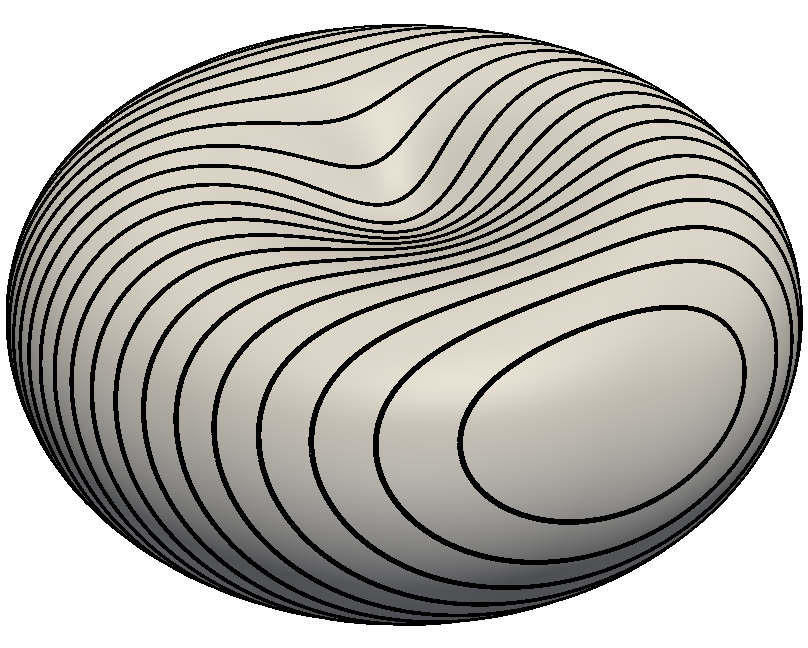
\includegraphics[width=0.24\textwidth]{pic/rbc/re_10/solution_0000.png}
		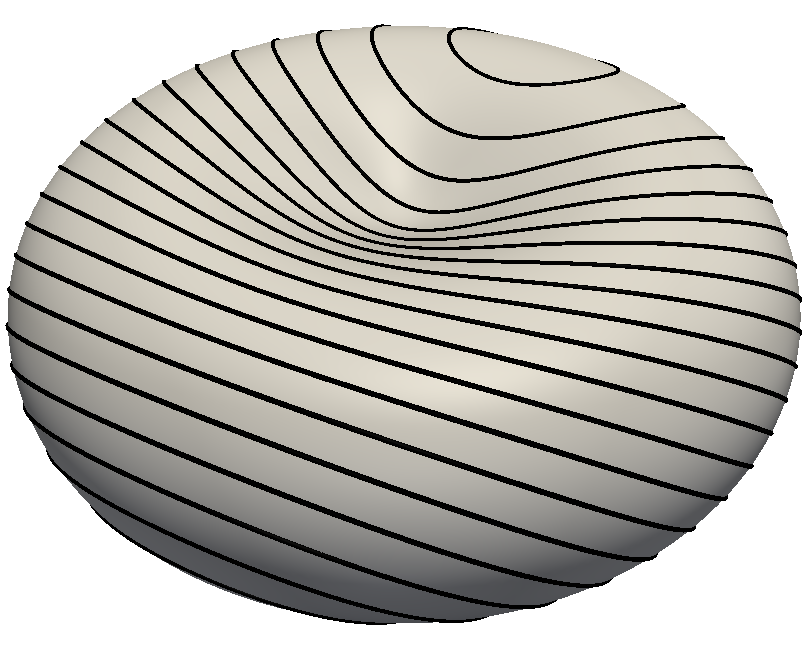
\includegraphics[width=0.24\textwidth]{pic/rbc/re_10/solution_0007.png}
		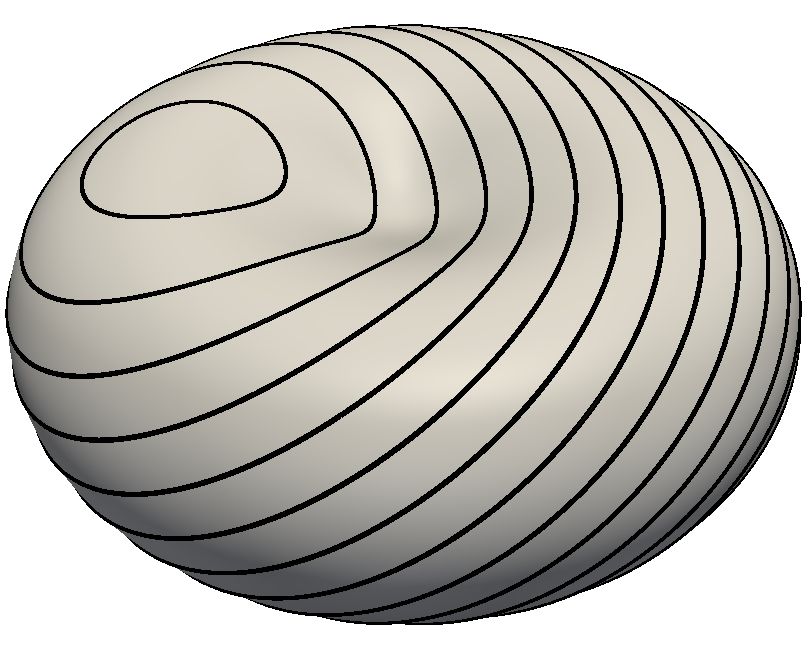
\includegraphics[width=0.24\textwidth]{pic/rbc/re_10/solution_0014.png}
		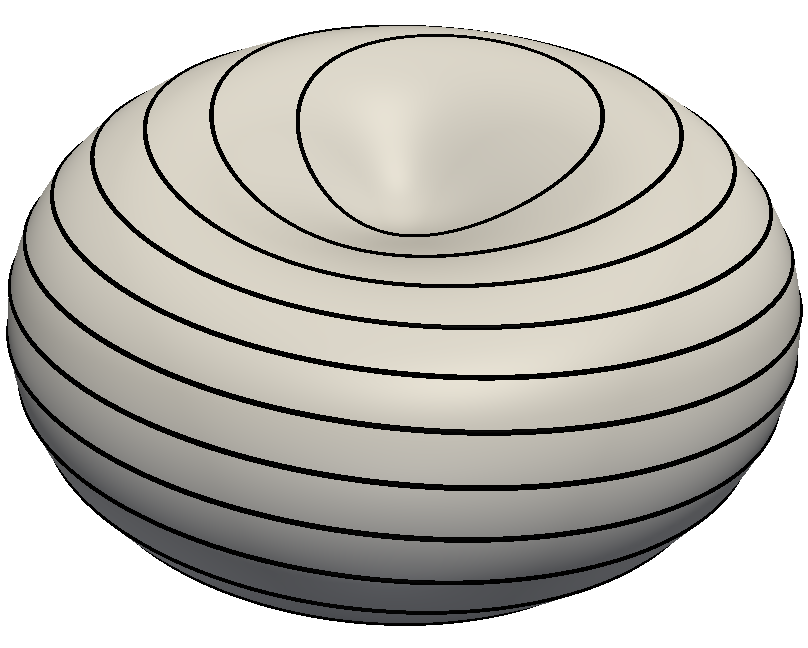
\includegraphics[width=0.24\textwidth]{pic/rbc/re_10/solution_0028.png}\\
		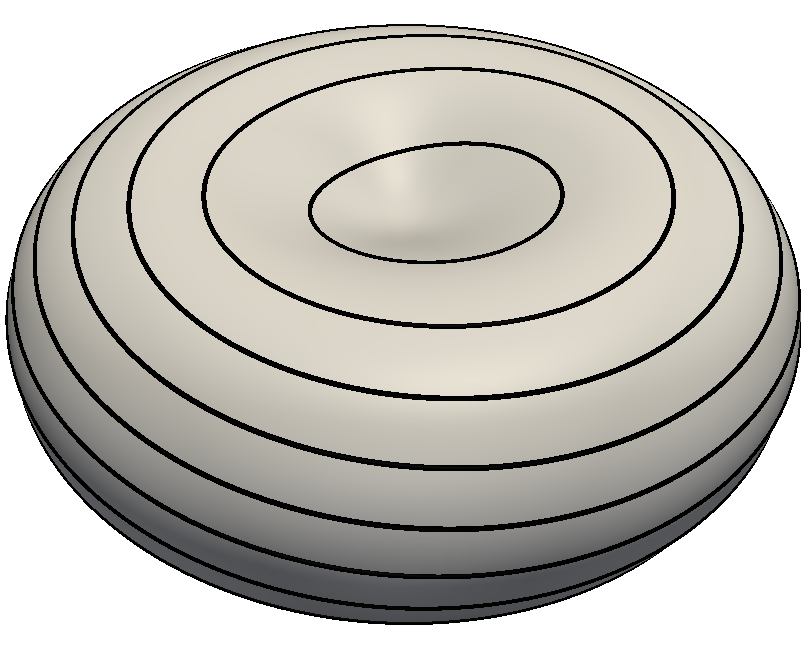
\includegraphics[width=0.24\textwidth]{pic/rbc/re_10/solution_0042.png}
		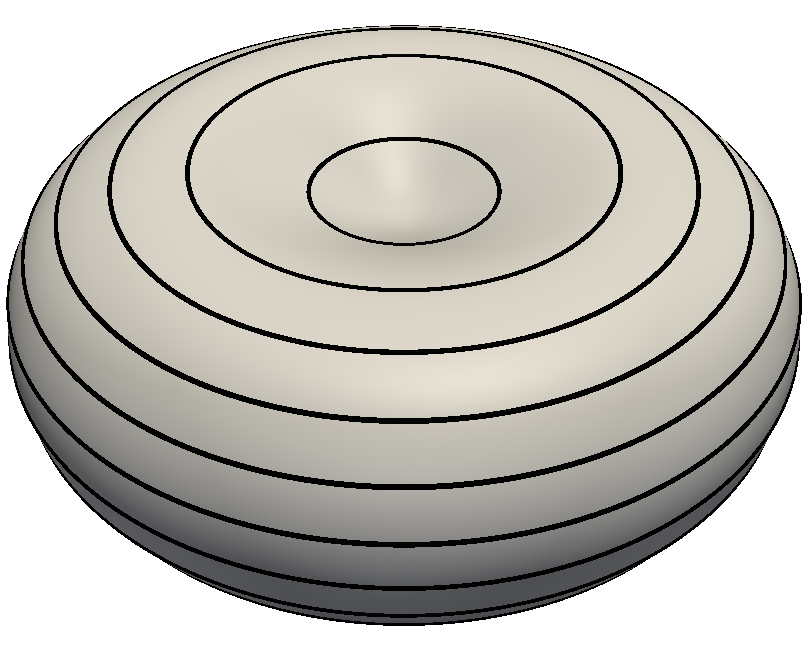
\includegraphics[width=0.24\textwidth]{pic/rbc/re_10/solution_0200.png}
		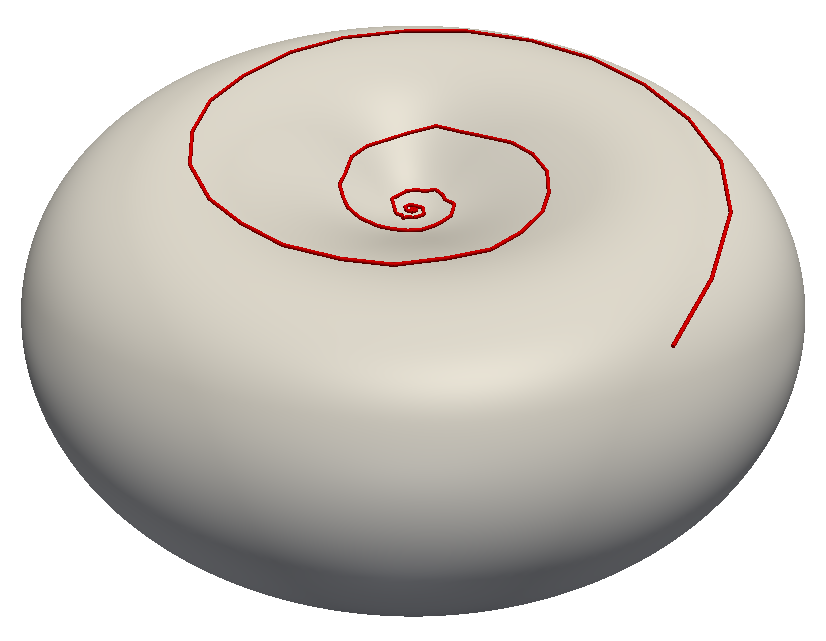
\includegraphics[width=0.24\textwidth]{pic/rbc/vortexTrack_re_10.png}
		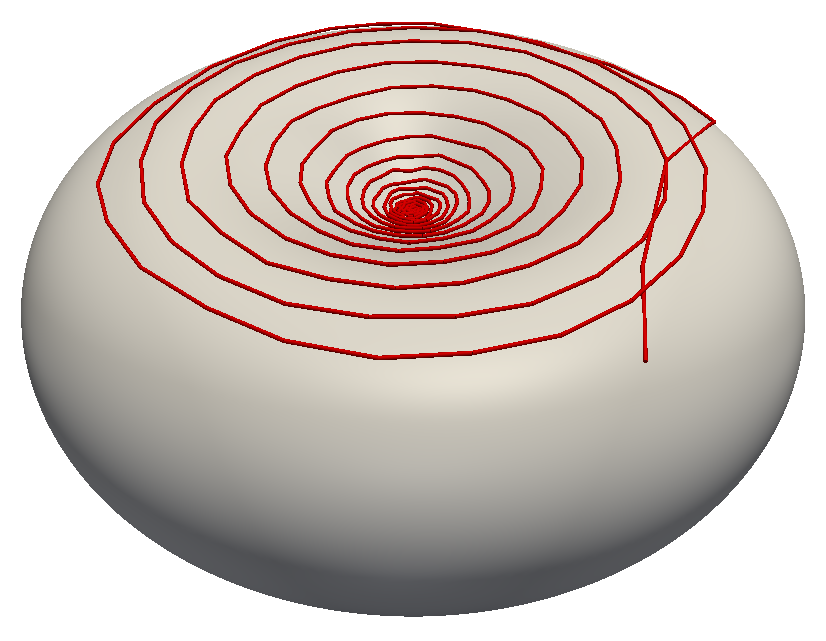
\includegraphics[width=0.24\textwidth]{pic/rbc/vortexTrack_re_100.png}
	\end{minipage} \\
	\caption{(left to right, top to bottom) Streamlines at $t = 0, 7, 14, 28, 42$ and $200$ for a rotating flow. Results are shown for $\text{Re}= 10$. 
    Vortex trajectories for $\text{Re} = 10$ and $\text{Re} = 100$.}
	\label{fig4}
\end{figure}
\begin{figure}[h]
	\centering
	\begin{minipage}{0.92\textwidth}
		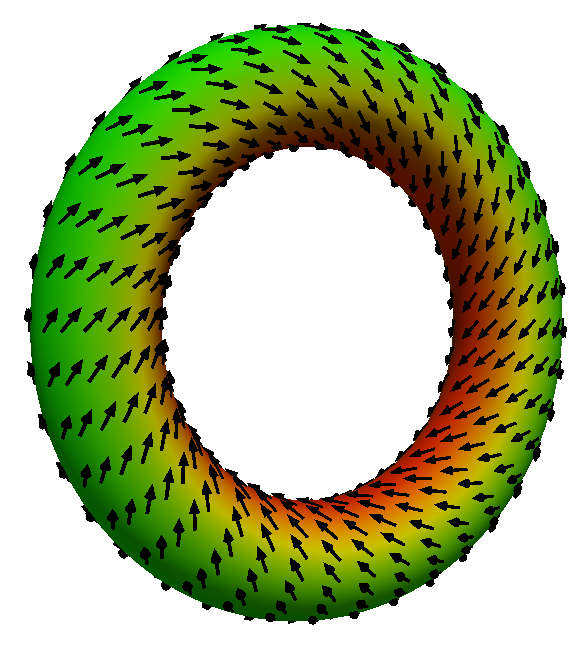
\includegraphics[width=0.19\textwidth]{pic/torus/re_10/solution_0000.png}
		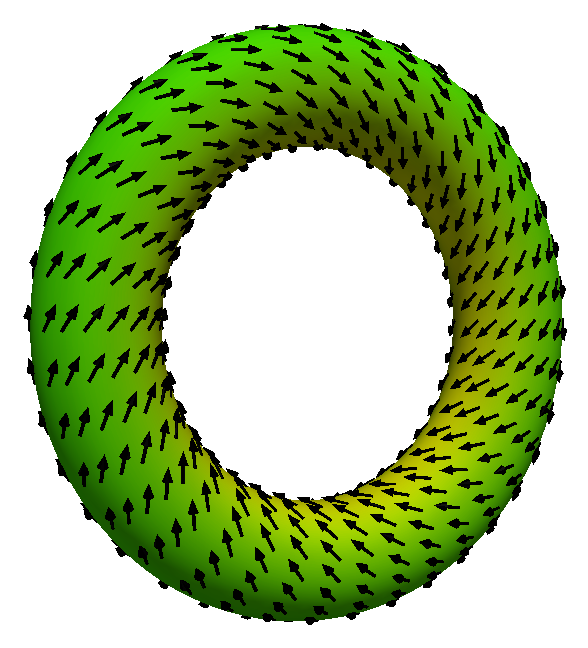
\includegraphics[width=0.19\textwidth]{pic/torus/re_10/solution_0002.png}
		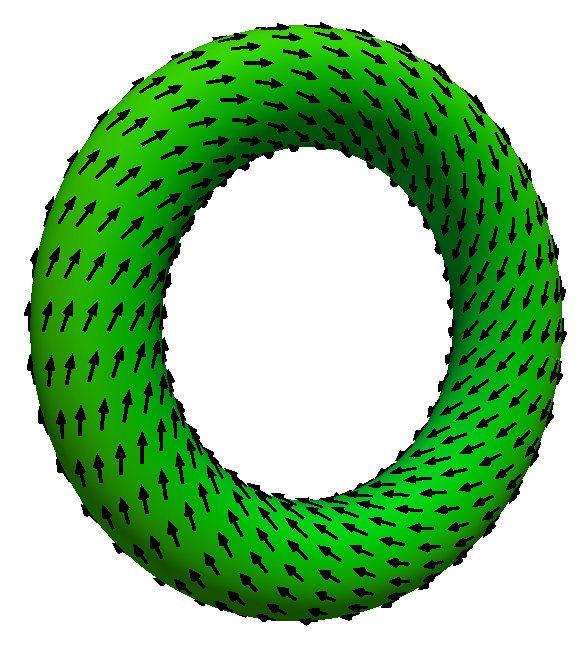
\includegraphics[width=0.19\textwidth]{pic/torus/re_10/solution_0010.png}
		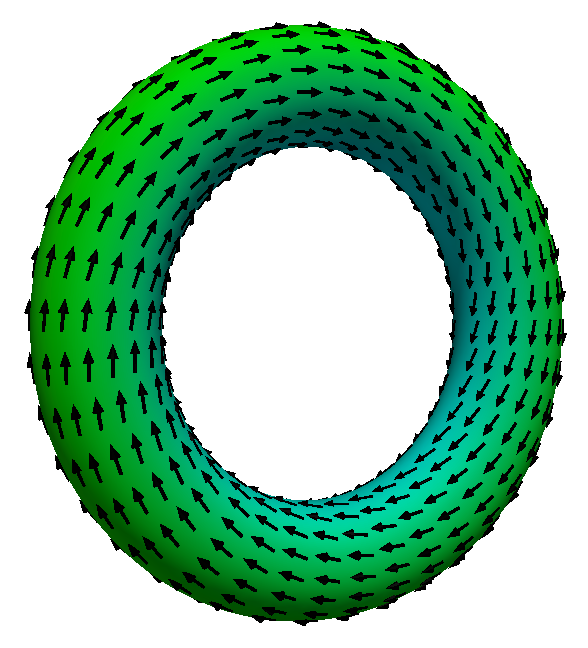
\includegraphics[width=0.19\textwidth]{pic/torus/re_10/solution_0030.png}
		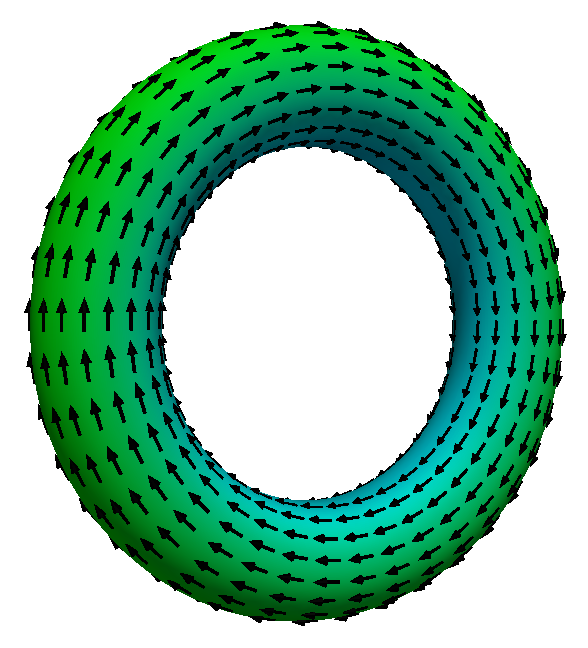
\includegraphics[width=0.19\textwidth]{pic/torus/re_10/solution_0060.png}
	\end{minipage}
	\begin{minipage}{0.06\textwidth}
		\centering
		$|\ub^{\sharp}|$\\
		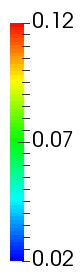
\includegraphics[width=\textwidth]{pic/torus/vColorbar.png}
	\end{minipage}
	\caption{Velocity field at $t = 0, 2, 10, 30$ and $60$ (left to right). We use a harmonic vector field \( \ub^{\sharp}_{0}\in\text{Ker}(*\exd*) \cap \text{Ker}(*\exd) \) as initial condition. 
  The arrows are rescaled for better visualization.}
	\label{fig:torus:2}
\end{figure}
\vspace{-6pt}%

\begin{thebibliography}{99}
\setlength{\parskip}{0pt}

\bibitem{Nitschkeetal_arXiv_2016} {Nitschke}, I. and {Reuther}, S. and {Voigt}, A.
Discrete exterior calculus (DEC) for the surface Navier-Stokes equation
{\it arXiv:1611.04392\/}. (2016).
\bibitem{Hirani_2003}Hirani, A.N.
  Discrete Exterior Calculus.
{\it Ph.D. thesis\/}. California Institute of Technology (2003).
\bibitem{Desbrunetal_arXiv_2005} Desbrun, M. and Hirani, A.N. and Leok, M. and Marsden, J.E.
Discrete Exterior Calculus.
{\it arXiv:math/0508341\/}. (2005).
\bibitem{ArroyoDeSimone_PRE_2009} Arroyo, M. and DeSimone, A.
Relaxation dynamics of fluid membranes.
{\it Physical Review E\/}. 79:031915, (2009).
\bibitem{Reutheretal_MMS_2015} Reuther, S. and Voigt, A.
The Interplay of Curvature and Vortices in Flow on Curved Surfaces.
{\it Multiscale Modeling \& Simulation\/}. 13:632--643 (2015).

\end{thebibliography}

\end{document}
